% Introduction

% ??? NEED block diagram of go()! check map? scan: yes/no? save map, move etc. (use that online code to block diagram tool)
% ??? Descripe framework in a section (see gdocs for input to block diagram) (or present at exam)
% ??? Mention we chose to focus on making our own code with the least use of finished libraries as possible, no error handling 
% ??? Mention the report will explain important aspects of out work and theoretical parts, 
%     while the finished product is a prototype and the code in the appendix
% 
% https://en.wikipedia.org/wiki/Rescue_robot
% Problem:
% - Problem and analysis:
% - System diagram (what we want to build):
% Daniel has already made a nice diagram of this

% Robot control: (maybe after pathfinding?)
% Theory:
% - functionality
% - step/control sequence
% Implementation: (programming)
% - programming/framework etc.

% Map handling:
% Theory (how we did and thoughts):
% - Introduction (what is map handling about, what have we covered here, problems we want to solve)
% - Analysis of map input6
% - Converting analog map to digital map (intro)
% - 
% Implementation:
% - Read, compare, update 

% read google docs

% Programming:
%- Data structure
%- Framework

\chapter{Map Handling}
\label{ch:map} % chapter label
The rescue robot should be able follow a given path from start to finish, based on a predefined map given as input.
A map provides useful information about whether areas of the map are accessible or not, which is important for path-finding.
Map data can be given to the robot prior to its physical presence at a location. Once the robot is at the starting point, it has to rely on its sensors for updated information about the surroundings.

A structured way of storing the required map data for different maps was designed. 
The goal was to not only make it readable by the microcontroller,
but also allow easy user input.

%Existing pathfinding algorithms such as Dijkstra and A* was studied, 
%in order to understand what input data such algorithms typically would require. 
%The pathfinding algorihtm implemented in this project is further described in chapter \ref{ch:path}.

\newpage
\section{Map Requirements}
\label{ch:map_requirements}
Maps can be found in a lot of different styles,
varying in how they represent specific informations.
Those styles often depend on the purpose of the map.
Figure \ref{sub:orient} shows a map for casual orientation purposes,
while \ref{sub:evac} shows a standardized evacuation plan.

\begin{figure}[h!tp]
    \centering
    \subfloat[Section of AAU Esbjerg]{%
        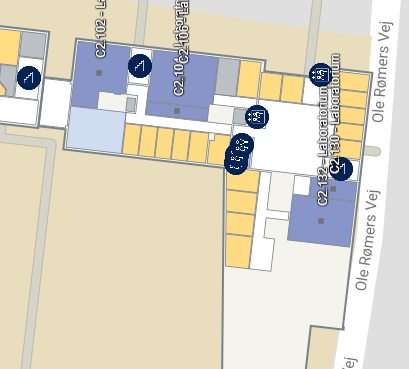
\includegraphics[width=0.4\textwidth]{figures/map/floorplan_aau.png}%
        \label{sub:orient}
        }%
    \hspace{0.1\textwidth}
    \subfloat[School layout example]{%
        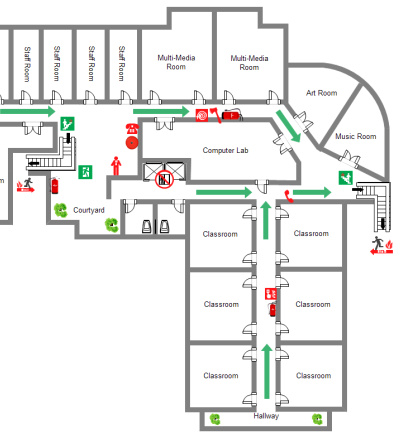
\includegraphics[width=0.4\textwidth]{figures/map/floorplan_school.png}%
        \label{sub:evac}
        }%
    \caption{Examples of different maps}
    \label{fig:floor_plans}
\end{figure}
% https://www.edrawsoft.com/school-layout-example.php

Maps are often very visual, providing a lot of detailed information to the reader.
The way the information is represented differently,
makes it very hard to be interpreted automatically.
A map must provide necessary information,
in a way that can be interpreted by the micro controller.
For this project we decided that a simplified map, would be sufficient.

Table \ref{table:map_data} shows the data the map should include,
as well as some areas that have been delimited from.

\begin{table}[h!]
	\centering
	\caption{Map data}
	\begin{tabular}{|p{0.4\textwidth}||p{0.4\textwidth}|}
		\hline
		Data to be included & Data to delimit from \\ 
		\hline
		Map dimensions 		& \parbox[t]{0.4\textwidth}{Differences in height\\(levels, stairs etc.)}\\
		\hline
		Start position 		& Door openings \\
		\hline
		Finish position 	& \parbox[t]{0.4\textwidth}{Ground surface\\(slipping, traction)} \\
		\hline
		Walls 				& Objects\\
		\hline
	\end{tabular}
	\label{table:map_data}
\end{table}


\section{Map Coordinates}
\label{sec:map_coordinates} % section label
During the theoretical development we often used hand-drawn 2D grid maps as depicted in Figure \ref{sub:2d_map}. The map can have a certain size, and it allows for any object to have a location on the grid, and can easily be referred to by its unique coordinate in the x and y dimensions. 

For converting such analog maps into a usable digital representation, we chose to use 2D arrays as data structure for storing maps. A 2D array can be thought of as a matrix, where a grid of numbers can be arranged in rows and columns. 2D arrays are very similar to matrices, and differs in how elements are indexed.

The result of the different indexing methods can be seen by comparing Figure \ref{sub:2d_map} to \ref{sub:2d_array}. Given the same index values, the cell referred to would be different, as seen in  Figure \ref{sub:2d_map} and \ref{sub:2d_array}.

\begin{figure}[htp]
    \centering
    \subfloat[2D grid map]{%
        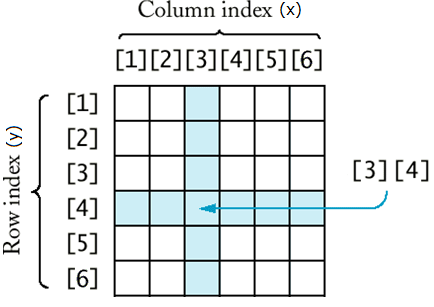
\includegraphics[width=0.45\textwidth]{figures/map/2d-map.png}%
        \label{sub:2d_map}
        }%  
    \hspace{0.05\textwidth}  
    \subfloat[2D array]{%
        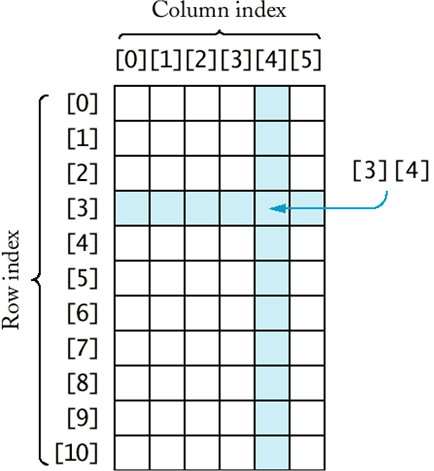
\includegraphics[width=0.45\textwidth]{figures/map/2d-array.png}%
        \label{sub:2d_array}
        }%
    \caption{Difference in indexing for (3,4) in a 2D grid map and a 2D array}
    \label{fig:floor_plans}
\end{figure}
%https://i.stack.imgur.com/tFdLk.gif

Each cell in the map represents a map segment with its own coordinate. To allow for a more logical access to segments of the map in the actual programming, we chose to start map coordinates at zero. Rows and columns could be switched when needed. This could be either be done in the syntax, by switching i and j, or by switching the x and y axes when storing the map in the first place.
\\

Example of looking up a map segment before switch rows and columns
\begin{lstlisting}[language=Python]
Array: map[4][3], would give map coordinate (3,4)
\end{lstlisting}

Example of looking up a map segment after switching rows and columns
\begin{lstlisting}[language=Python]
Array: map[3][4], would give map coordinate (3,4)
\end{lstlisting}

This lead to the final implementation in our program using 2D arrays, 
where the value of any given map segment could easily be found. 
\\
Example of implementation in the final code
\begin{lstlisting}[language=Python]
Array: robot->map->segments[3][4], would give map coordinate (3,4)
\end{lstlisting}
More examples of this can be seen in the final code in appendix XX, XX, and XX. 
The same approach was used for handling node maps, which is further explained in section X.

\section{Map Design}
\label{sec:map_design} % section label


Subsections?\\
- map design (show the map + wiki?)\\
- read, update, write? (dynamic/malloc / dimension)(refer to code?)\\
- explain neighbours / wall hex\\
- explain node map\\
%Explain we made the map size dynamic to handle any map size\\
%Explain how to store wall as hex value?\\

%- framework?

\begin{figure}[htp]
    \centering
    \subfloat[ASCII]{%
        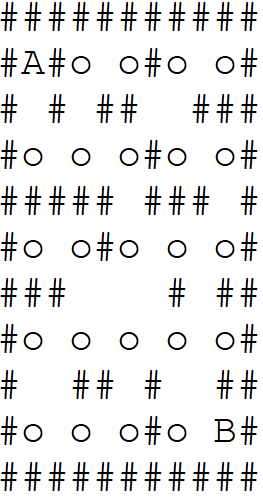
\includegraphics[width=0.2\textwidth]{figures/map/5x5map_ascii-2.png}%
    }
    \hspace{0.2\textwidth}
    \subfloat[UTF8]{%
        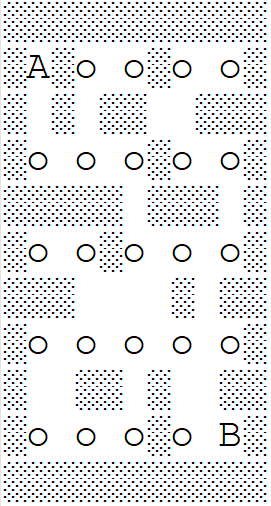
\includegraphics[width=0.2\textwidth]{figures/map/5x5map_utf8-2.png}%
    }
    \caption{5x5 map}
    \label{fig:5x5map}
\end{figure}

\section{Check Map}
\label{sec:map_check} % section label
Remember we have a chapter dedicated to scan.\linebreak
Based on scenario things might have dramatically changed, even to the point of map being useless. Explain how map is updated.

\section{Implementation}
\label{sec:map} % section label
Code here, or parts of code under each section?\\
Code here!
\\
Like with many others,
is the first step in Dijkstra's algorithm to reduce the map to the necessary minimum.
After this reduction, the map only consists of \emph{nodes} and \emph{edges}.
An edge connects two nodes together and has one integer \emph{travel cost}.
In this integer is stored how much it costs to traverse along that edge,
measured in the metric that should get optimized (in our case distance).


